\section{Validation des modèles}


\subsection{Classification supervisée}
Afin de mettre place des modèles utilisables et de qualité certaine, nous utiliserons la classification supervisée.\\
Nous nous attaquerons donc en priorité à l'union européenne et tacherons de vérifier si les résultats sont probants.

\paragraph{Global}
Dans un premier temps, nous étudierons si il est possible de reconnaitre un pays de l'Union Européenne en se basant sur l'ensemble des critères disponibles dans le jeu \jeuc .

\paragraph{Santé}
Il nous semble intéressant de vérifier si l'on peut déterminer si un pays est membre de l'UE en se basant sur les seuls critères de santé.\\
Nous nous appuierons donc sur des arbres de décisions pour permettre cet apprentissage.
\begin{figure}[H]
	\begin{center}
		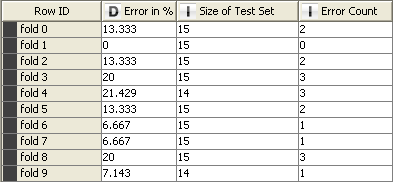
\includegraphics[scale=0.5]{Image/ErrorRatesSante}
		\caption{Resultats de la CrossValidation de l'apprentissage des Membres de UE sur les critères de santé}
	\end{center}
\end{figure}


